\documentclass[a4paper]{article}

\usepackage[utf8]{inputenc}
\usepackage[T1]{fontenc}
\usepackage{textcomp}
\usepackage[english]{babel}
\usepackage{amsmath, amssymb}
\usepackage{listings}
\usepackage{physics}


% figure support
\usepackage{import}
\usepackage{xifthen}
\pdfminorversion=7
\usepackage{pdfpages}
\usepackage{transparent}
\newcommand{\incfig}[1]{%
	\def\svgwidth{\columnwidth}
	\import{./figures/}{#1.pdf_tex}
}

\pdfsuppresswarningpagegroup=1
\title{CS 766 - Analysis of Concurrent Programs}
\begin{document}
\section{Introduction}
Taking notes from the first recorded lecture. The speaker says that
this is about what to expect from the \textit{second  part of this course}.

Most modern processor architectures are multicore - threads can be
executed in parallel. Other than architecture level concurrency,
distributed computing systems, e.g. databases, involve concurrent
execution so that any one node can provide a coherent and uniform
picture of the database irrespectively of where you are in the world.

Support for concurrency
\begin{itemize}
	\item architecture level
	\item distributed systems
	\item programming languages (modern standards of C++, Java etc, modern languages like Rust)
\end{itemize}

Naming conventions
\begin{itemize}
	\item Shared variables: \texttt{x, y}
	\item Local variables/registers: \texttt{a, b, c, d}
\end{itemize}

Consider two threads 
\begin{table}[h]
	\centering
	\caption{initially \texttt{x = 0}}
	\label{tab:ex1}
	\begin{tabular}{c || c}
		$th_1$ & $th_2$ \\
		\texttt{x:=1} & \texttt{x:=2} \\
		\texttt{a:=x} & \texttt{b:=x}
	\end{tabular}
\end{table}

Traditional semantics used to implement concurrent programs - sequential
concurrency (SC). From what I understood, this means that two threads
cannot be interleaved; execution of one thread cannot be interrupted
by a ``context switch".
You always read from the latest possible write. It was summarized in the
lecture as
\begin{itemize}
	\item Shared memory
	\item Processes/threads: atomic read/write
	\item interleaving of operations across threads
	\item simple, but too strong
\end{itemize}

Too strong? If you look at modern system designs - mircoprocessors, cache protocols,
distributed computing don't use SC, but use weak memory models instead.

\begin{itemize}
	\item Intel: TSO
	\item IBM: Power
	\item ARM
\end{itemize}

As for programming languages
\begin{itemize}
	\item C11
	\item Java
	\item Rust
\end{itemize}
provide first-class support for concurrency use release-acquire semantics,
which is also a weak memory model. The
behaviour of your program under this semantics will be different from
what you can expect for sequential consistency.

Consider the example of a simple program. Init: \texttt{x=y=0}.
\begin{table}[h]
	\centering
	\caption{two threads}
	\label{tab:ex2}
	\begin{tabular}{l l}
	\texttt{x=1;} & \texttt{y=1;} \\
	\texttt{ry=y;} & \texttt{rx=x;}
	\end{tabular}
\end{table}

[Second sitting begins here. Will not try to make notes for everything
that the speaker says - only handful of important points]

In the above threads, using SC cannot yield a state where both \texttt{rx} and \texttt{ry} are \texttt{0}. On the other hand, if we allow
``context switches" between a thread execution, i.e. under release-acquire
semantics, we can reach a state where \texttt{rx=ry=0}.

Different memory models allow different  constraints for how threads
can be interleaved. General class - weak memory models.

In RA semantics - release writes, acquire reads (look up on your
fave search engine). 

\textbf{Reachability problem:} Consider a general multithreaded program with a bunch of shared
resources and local variables. The question we are interested in -
\emph{is this program unsafe?} Is it possible to reach a bad state?
(Under some semantics). Can we write an algo that can tell whether
such a bad state is reachable?

So, we want to build a tool that takes a concurrent program as an input
The problem could be either decidable or undecidable. If it the reachability
is determinable, then there'll be some complexity and all that shebang.

The other aspect is ensuring that a bad state  can never be reached.
Of course, we cannot really go about exploring all possible reachable
states. There should be a way of ``pruning the search".

So, a process $\pi$ is a sequence of instructions. There is another
abstraction - trace $\tau$. A trace is essentially a  graph. Each
node is an atomic instruction. Edges can be
\begin{itemize}
	\item \texttt{po} - program order
	\item \texttt{rf} - read-from
	\item \texttt{co} - coherence order
	\item  \texttt{fr} - from-read
\end{itemize}

SC is guaranteed if the graph is acyclic. We say that $\pi \models \tau$ 
(read as ``pi models tau").

Once you have a particular trace, you can look at different processes
$\pi_i$ to see whether they are consistent with the trace.

We explore the program by generating and exploring traces. Sufficient
to explore one run per trace to verify. In general multiple runs correspond 
to a single trace.

\begin{figure}[h]
	\centering
	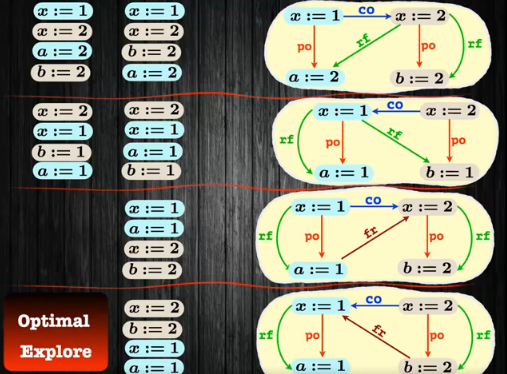
\includegraphics[width=0.8\textwidth]{figures/traces.png}
	\caption{Example of exploring using traces}
	\label{fig:figures-traces-png}
\end{figure}


\section{Some Self Study}
This section is comprised of notes taken while reading from Shavit et
al.

Gotta start thinking like a concurrent programmer - understanding
when operations ``happen", identifying all possilbe interleavings etc.

Two complementary directions
\begin{itemize}
	\item Principles - computability, what can be computed in an asynchronous concurrent environment
	\item Practice
\end{itemize}

Consider the example of finding all prime numbers $< 10^{10}$,
and you have ten threads at your disposal. A naive approach would be
to distribute the input domain between all threads equally, but this
would be far from optimum given how load balancing is affected.

An alternative would be to use a shared counter and assign an integer
to each thread.
\lstinputlisting{listings/sharedcounter.cpp}  % is actually java btw

Note that the above implementation of the shared counter is a bit
naive, because the instruction \texttt{return value++;} is actually
something like

\texttt{long temp = value;}

\texttt{value = temp + 1;}

\texttt{return temp;}

\texttt{value} is shared. \texttt{temp} is local. 

Modern microprocessors have hardware support for atomic instructions that
update shared counters etc (mutex?). Alternatively a software solution would require
ensuring that only one thread updates the shared variable before another
thread can do anything with it. E.g. Rust compilers should be able to do this
statically. This is a classic problem in multiprocessing algorithms,
called the \textit{mutual exclusion problem}.

I've heard some of these terms before
\begin{itemize}
	\item mutex
	\item deadlock
	\item bounded fairness
	\item blocking vs non-blocking synchronization
\end{itemize}

\section{First Lecture}
The course is about software verification, specifically concurrent software.
Very open problem. Situations can be decidable or undecidable. 

The technology is getting there, but it's not \emph{there}-there.
If you want to verify that your software, you know, works, it's not
as straightforward as just downloading a verification tool and reading
its API documentation. You need a whole team that understands the
whole verification shebang.

Even if you have only two threads, the situation can become significantly
more complicated than a similar sequential situation. Rust was made
because most bugs on Firefox were concurrency bugs.

\textbf{Question:} What is the number of schedules between two threads
with number of instructions $N_1$ and $N_2$? 
\[
	^{N_1+N_2}\text{C}_{N_1}
.\] 
i.e. context switches can happen anywhere. \emph{Blowup}

A lot of things can go wrong
\begin{itemize}
	\item synchronization primitives - sets of allowed schedules
		appear deceptively simple, but are ugly AF
	\item how would you go about formally proving that a concurrent
		program is actually corrent?
	\item deadlocks and all that.
\end{itemize}

\subsection{Summarize interleavings}
One should be able to efficiently summarize valid interleavings.
Four techniques
\begin{itemize}
	\item environment computations - e.g. if shared $g>0$, some
		thread increases $g$ by 2.
	\item Sequentialization (Code transformation)
		\begin{itemize}
			\item merge code of thread 1 and 2 such that the merged code is equivalent to the original code
		\end{itemize}
	\item Happens before summaries
		\begin{itemize}
			\item enforcing ordering contraints between
				different instructions in different threads?
		\end{itemize}
	\item Bounded-context switches
		\begin{itemize}
			\item most reported bugs have at most 2-3 context switches. If a bug is there in the code, it will be discovered in a couple of interleavings. Hmmmmmmmmmmmmmmmmmmmmmmmmmm.
			\item tools based on this idea have actually
				been very  successful
			\item I would guess that this does not cover
				edge cases - they are not well-documented anyway. reporting bias comes into play
			\item this bias is why such solvers are winning
				in verification competitions - benchmarks
				don't include those edge cases
		\end{itemize}
\end{itemize}

An example of a (very dumb) queue is given. Enqueue and dequeue operations happen
concurrently. Enqueue should be fine. Dequeue will be nontrivial.
For  the time being let's not worry  about blowing the stack.

You have thousands of threads performing these two operations  on this
shared structure concurrently. What even is FIFO here? A paper in 1995
formally showed correctness of this. That even in this massively concurrent
environment.

\textbf{prerequisites:} logic for computer  science.

\textbf{Weekly Moodle quizes } - twice a week maybe policy TBD

\textbf{Conferences:} POPL etc
\end{document}
